\documentclass[12pt, english, NoHyper]{AE4010-template}
\usepackage[]{natbib}
% \usepackage[sorting=none, citestyle=numeric-comp, natbib=true]{biblatex}    % For numbered biblatex references
%  \usepackage[citestyle=authoryear]{biblatex}      % For author year biblatex references
\usepackage{csquotes}
\usepackage{hyperref}
\usepackage{amsmath}
\usepackage{graphicx}


%% Uncomment the following three lines when using the biblatex package
%\bibliography{bibliography.bib}
%\addbibresource{bibliography.bib}
%\bibliography{apa}
%% Uncomment the following line when using the natbib package
\bibliographystyle{plainnat}





%% Define your title entries here
\title{Identification of Potentially Hazardous Asteroids}
\author{J. G. P. Vermeulen}
\yourstudynumber{4382889}
\yourmscprofile{Space Flight}
\yourmsctrack{Space Systems Engineering}









%   ########################################################################
%               PLEASE COMPILE USING XELATEX FOR THE BEST RESULTS
%   ########################################################################









\begin{document}
\maketitle

\section*{Executive Summary}
In this section try and state, in under 300 words, the major aspects of your project plan. It should include what the project is about, what the main content of the plan will be what the main objectives of your research are, the methods you will use to achieve those objectives and what your possible findings could be. End with a strong sentence that highlights the significance of the work to be undertaken and any long-standing contribution to the body of knowledge. Remember that this is a proposal of work to be done and so you might also say something about the motivation and feasibility.





\section{Introduction}
In recent years, human efforts have catalogues all very large near-Earth asteroids and determined none of these to be a threat in the foreseeable future. However, as illustrated by recent impacts such as the Chelyabinsk and Tunguska meteors, smaller, unknown, asteroids still pose a significant threat to human life and property. In addition, an upscaling of Earth-based detection methods will not suffice to safeguard humanity from these natural disasters: unfavorable phase angles and atmospheric interference make detection from the Earth inefficient (\cite{DefendingPlanetEarth}). In recent years, a multitude of studies (e.g. \cite{NEOSDT1}, \cite{ThesisOlga}) have been performed to assess the effectivity of a future space-based Near-Earth Object surveying mission. These studies have yielded promising results, but still suffer from some additional issues, such as interference my sunlight and limitation on data processing. Therefore, a system of detection is proposed based on autonomous satellites placed strategically in the solar system to automatically detect near-Earth asteroids and identify whether these are impact-hazardous to Earth. \\

This work contains a project plan for proposed research into the topic of multi-satellite asteroid surveys. Firstly, an overview of the current state of literature, and the position of the work therein is discussed. Next, the core of the research as intended is described, starting with the research question, aim and subgoals; followed by the methodology, setup of the experimentation, and expected outcomes. Lastly, a short discussion of the project plan will be given.







\section{State-of-the-art/Literature Review}
Study of Potentially Hazardous Asteroids (PHA's) began through initiatives from governments to safeguard Earth from the threat of asteroid impacts, resulting in several of the foundations of the field (\cite{InitialTaskforce}, \cite{DefendingPlanetEarth}). These agreed upon the initiative to identify 90\% of all Near-Earth Asteroids\footnote{Defined as an asteroid with perihelion < 1.3 AU} larger than 140 m in diameter. This was based on the calculation that this would eliminate 90\% of the remaining background risk. Thus, the PHA was defined as an asteroid with a diameter over 140 meter, which intersects Earth's orbit within 0.05 AU. \\

In the following years, a multitude of surveys were carried out to achieve this goal, such as, but not limited to, the Catalina Sky Survey and the PANSTARRs survey in Hawaii. In addition, several surveys were carried out from space, most notable the NEOWISE survey which repurposed the WISE imager after its main cryogenic payload had run out. The performance of these surveys has been spectacular (see e.g. \cite{NEOWISEFlex}). However, as shown by \cite{PopulationHarris} in \autoref{fig:populationdifference}, a large fraction of asteroids is still unknown.\\

\begin{figure}[thb]
 \centering
 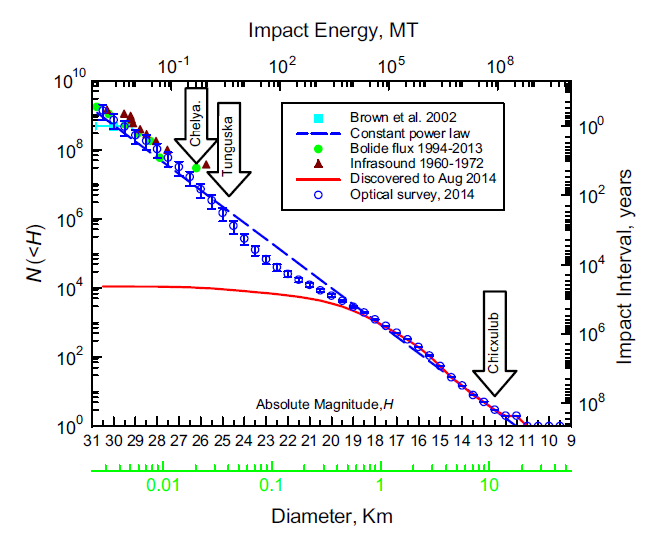
\includegraphics[width=0.8\textwidth]{figures/populationdifference.png}
 \caption{Relationship between asteroid absolute magnitude (and thus size, and impact energy) to their occurence. Shown are the expected population of these asteroids, compared to the number discovered in contemporary surveys.}
 \label{fig:populationdifference}
\end{figure}

As the remaining fraction of asteroids not only poses a threat to human safety and property, but discovering them will also yield valuable scientific insights into the structure and origin of our solar system (\cite{Populations}), a number of new surveys is currently being researched and developed. Among the ground-based surveys, the most impressive project is the Large Synoptic Survey Telescope at the Vera C. Rubin observatory in Chile (see \cite{LSST} for a thorough overview). However, as Earth-based surveys are limited by weather, day/night cycles and atmospheric dispersion, most of the research is focussed on space-based surveys. \\

Although the efficacy of Earth-orbiting missions has already been shown by missions such as the Spitzer space telescope and NEOWISE, there is currently a lot of interest in deep space surveys. Advantages of these surveys include not being influenced by sunlight reflected off Earth, more favourable viewing angles, and greater relative motion to the asteroids (\cite{NEOSDT1}). The largest barrier to performing these missions, the lack of sufficient computational power, has been resolved by advances in semiconductor technology. However, because of the vast costs of a space mission, most work is currently focussed on simulating surveys to determine optimal conditions, such as the work done at the European Space Agency by \cite{Flyeye} and at NASA Jet Propulsion Laboratory by \cite{NEOSDT2}. \\

Investigation of the possibilities yields that space-based surveys will be superior the current Earth-based surveys. Commonly researched orbits are Earth-Sun L1, Venus-Sun L1, Venus-trailing, and several Earth orbits, using either visual light or thermal infrared telescopes. \cite{ThesisOlga} expands on thes even further by showing advantages of using solar sails for more complex orbits. Although the performance of these surveys is impressive, there is still a large number of PHAs that will not be found by these surveys, and an even larger fraction of smaller NEOs that will remain undiscovered, as shown by \cite{NEOSDT2} in \autoref{fig:surveycompleteness}. Therefore, in this report, a proposal will be made to research if the performance of these surveys can be improved through utilization of a system of several satellites, hoping to exploit a greater variety in orbits, payload combinations, and viewing angles.

\begin{figure}[thb]
 \centering
 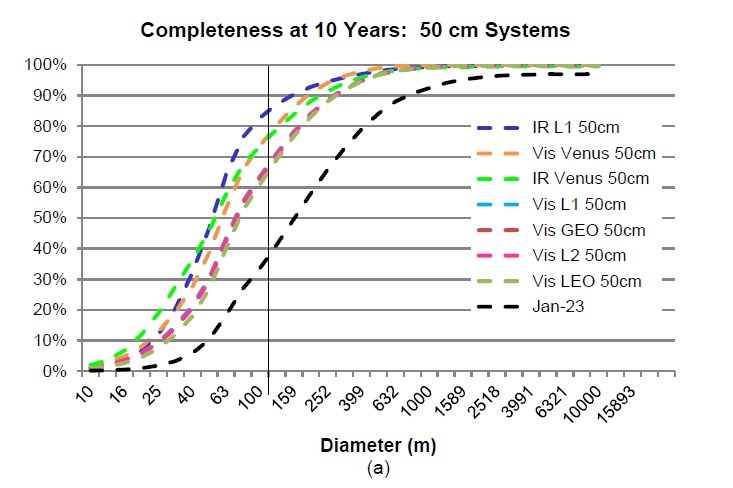
\includegraphics[width=0.8\textwidth]{figures/surveycompleteness.png}
 \caption{Survey completeness at 10 years, using 50cm telescopes.}
 \label{fig:surveycompleteness}
\end{figure}


\section{Research Question, Aim/Objectives and Sub-goals}
As there is currently no established baseline for multi-satellite asteroid surveys, the research will focus on examining how such a survey would compare to existing, more well studied proposals.

\subsection{Research Question}
Therefore, the research question of this work is:

\begin{quote}
 How is the performance, optimal position and configuration of a space-based system with the purpose of identifying and cataloguing near-Earth objects affected by the number of spacecraft in the system?
\end{quote}

As briefly alluded to previously, there are actually two objectives of such a survey: raising the ``survey completeness'', i.e. what fraction of asteroids is known, and raising the warning time for impactors heading towards Earth by identifying them early. Therefore, the following two sub-questions are identified:

\begin{quote}
 How does the number of said spacecraft affect a system with the purpose of raising the warning time for Earth impactors?
\end{quote}
\begin{quote}
 How does the number of said spacecraft affect a system with the purpose of raising the survey completeness of near-Earth asteroids?
\end{quote}

And lastly, a tangential question that will be a crucial component of the main project:

\begin{quote}
 What is the influence of a system utlizing mixed infrared and visual telescopes to perform said survey?
\end{quote}

This final question is often suggested as future work by authors (e.g. \cite{AsteroidsInTIR}, \cite{AsteroidSTM}), and should be investigated independently to ensure a proper interpretation of the configuration of the system.

\subsection{Research Objective}
As mentioned previously, modern research into this topic is carried out through detailed modelling of surveys using computers. Therefore, the main research objective of this thesis is:

\begin{quote}
To investigate the influence of the number of satellites in a space-based survey through detailed simulation of near-Earth asteroid surveys.
\end{quote}

The first of the sub-objectives is to accurately model the asteroid population. Several alternatives exist for this, but it is important to consider the implications of how the models were constructed, given that none of them was based on a deep space survey.\\

The second sub-objective is to accurately model the survey of this population. For this, three issues have to be addressed: Firstly, the signal generated by the asteroid has to be modelled. Secondly, the background signal and noise has to be modelled. With these two objectives completed, a suitable survey cadence should then be derived to integrate the survey in time.\\

Lastly, the ``optimal'' part of the survey. As the satellites are not bound to a single position, options such as L1 points are no longer a de-facto preferred location. Therefore, a method is necessary to determine what the optimal placement and composition of such a system is. Most likely, this will be the most computationally intensive part, as the complexity of the problem quickly grows when increasing the size of the system.

\section{Theoretical Content/Methodology}
In this section, the methodology for the three sub-objectives stated above is laid out. Furthermore, as a complicated model is to be developed, there will also be an addition of the methodology for validating said model.

\subsection{Asteroid Population}
%https://www.mv.helsinki.fi/home/mgranvik/data/Granvik+\_2018\_Icarus/
%https://www.sciencedirect.com/science/article/pii/S0019103517307017?via\%3Dihub#fn0003
Several peer-reviewed and validated models of the NEA population exist, which can be used easily for the intended research. It is important to assess the model using different population models, to ensure generalization of the solution. For a full population model, intended to assess the identification and cataloguing performance, two models have been selected. The first model is the de-biased model by \cite{PopulationGranvik}. This model continues on the work of \cite{PopulationHarris}, as well as the results of the NEOWISE mission. It derives an algorithmic model which can directly generate a representative population of NEA's. In addition to this model, the real database of NEAs gathered by NASA/JPL will be used (\cite{CNEOSDatabase}). Although this model is biased, as it only includes asteroids that were discovered already, it is known to be a correct representation of reality, as it is not simulated.\\

As asteroid impacts are rare, assessing the warning time requires a population of synthetic impactors. Using various methods, several authors have created and succesfully used populations of synthetic impacts, with representative orbital elements to actual impactors. The standard among these models is the model by \cite{ChelseyPop}. This model includes orbital elements for a large population of asteroids, as well as predicted time of impact. In addition, the model developed by \cite{Flyeye} will be used, which has been applied in this fashion in the past as well (see \cite{ThesisOlga}).\\

Lastly, in order to determine the position of the asteroids in time from their orbital elements, simple Keplerian orbits will be used, as precise accuracy of the orbits is not neccessary for the inteded research. This will save a lot of computational power in optimization.


\subsection{Survey Modelling}
Modelling of the survey is by far the largest part of the initial set-up work. The survey can be split up into three categories: Modelling the background signal and noise, modelling the signal from the asteroids, and modelling the cadence and detection by the satellite. As mentioned previously, both visual light and thermal infrared will be considered. Therefore, models needs to be developed for both.

\subsubsection{Background Signal and Noise}
There are a lot of components to the background signal: Diffuse starlight from the night sky, a concentration of background light along the plane of the Milky Way, the direct light of the Sun, the zodiacal light, and the so-called gegenschein. For simplicity, these components are split into a Solar and a galactic component. The Solar component is dependent on the location of the satellite around the Sun; the galactic component is not. \\

For the visual light, implementation is simple. Detailed measurements have been taken of the visual background light, see e.g. \cite{LightOfTheNightSky}. These values have been tabulated by \cite{DiffuseSkyBrightness}, split into Solar and galactic components. These can be directly implemented. \\

The thermal infrared signal is slightly more complicated, as the contribution of zodiacal light is dependant not only on reflection, but on temperature distribution of interplanetary dust. The most complete model available currently is based on the COBE mission, as described by \cite{COBEIRBackground}. This model is split up into detailed measurements of the galactic IR background, combined with a model of interplanetary dust. This model can be integrated numerically to find the contribution of interplanetary dust and solar radiation. \\

Lastly, there are several noise terms integral to the detector. These are mainly read noise and thermal noise. The values for these are hardware dependent and were taken from \cite{NEOSDT2}. In addition, because of the nature of a signal consisting of individual particles, there is a contribution of Poisson noise in all terms.

\subsubsection{Target Signal}
Determination of the target signal in the visual light is straightfoward: by assuming the asteroid approximates a lambertian sphere, and the stard phase function can be used. However, no such phase function has been found in the infrared spectrum. The basis for the infrared signature of an asteroid was given by \cite{AsteroidSTM}: By making an assumption on the temperature distribution of the asteroid, based on its thermal balance, a numerical integration of the visible hemisphere is performed for the flux. This model was later refined by \cite{AsteroidsInTIR} using data from a larger number of asteroids. Their Near-Earth Asteroid Thermal Model (NEATM) will be used in the experiment.

\subsubsection{Cadence and Detection}
Detection of NEAs is contingent on several repeat measurements. These \textit{tracklets} can then be combined to fit the orbital elements (\cite{OpNav}). Therefore, how often a measurement is taken is of relevance. In order to determine the frequency of measurements, the \textit{cadence}, an analysis of the ADCS will be performed together with the required integration time of the camera (from \cite{NEOSDT2} and \cite{ThesisOlga}). \\

To establish a detection, a signal-to-noise ratio calculation will be performed. This saves a lot of computational load compared to processing generated images. The SNR can be calculated according to \cite{NEODetection} as follows:
\begin{equation}
\mathrm{SNR} = \frac{\frac{1}{hc}A\tau k_{sf} \int_{\lambda_1}^{\lambda_2}E_A(\lambda)Q_e(\lambda)T(\lambda)\lambda d \lambda}{\sqrt{S_e + B_e + D_e + R_e^2}}
\end{equation}
With target and background signal in electrons $S_e$ and $B_e$, dark noise $D_e$ and read noise $R_e$. The remaining terms are largely efficiency terms, the interested reader is refered to \cite{NEODetection} or \cite{OpNav} for a thorough explanation. Note that only the poisson component of the background signal has to be taken into account, as the mean signal can be subtracted easily (\cite{OpNav}).\\

To convert a SNR to a detection, a probabilistic approach is taken. A lower threshold of SNR = 1 is set (0\% chance of detection), and a higher threshold of SNR = 5 (100\% detection). Between these thresholds, an integrated Gaussian is used to determine the detection probabilistically. 3 detections within a time span of 90 days will lead to the asteroid being identified (\cite{NEOSDT1}). Lastly, by numerically working through this model in time, the performance of the full asteroid survey can be modelled.

\subsection{Optimization}


\subsection{Validation}


\section{Experimental Set-up}
What is your laboratory set-up or in the field set-up? Present it such that readers can better informed and critical of any limitations of your research environment and your set-up. For example, how will the collaboration with industry work? Or are there any practical implications of your Methodology from Section 3? Keep in mind that Experiments are more than just questionnaires, interviews or physical tests in a laboratory. Creating or modifying a computer programme or a computer model is also considered an experiment, so their set up, documentation and limitations should be discussed here. 

Do not forget to include technical details such as machines to be used, programming language or modelling software and why you selected those to reach your objective as stated in section 3.




\section{Results, Outcome and Relevance}
What data etc. will you be working with, which variables and parameters, and what type of results do you want to investigate? Then go on to try and project the sort of outcome you are interested in and of course ultimately what the relevance of that is both for your project but try and say something about possible larger impacts of your work. Mention how you expect to validate and verify your results. This is a key part of your thesis, so it is important to consider this early in your research.





\section{Project Planning and Gantt Chart}
Look at the logistics of carrying out the work, develop the intended work into work packages (from the tasks mentioned in Section 3) and then incorporate all that into a schedule of work through a Gantt chart (or Integrated Master Plan/Integrated Master Schedule). You must, at a reasonably high level, try to estimate time required and any resource constraints etc. and then fit that into a schedule. A Work Breakdown Structure and Work Flow Diagram can be very helpful (ref: DSE). You will put in three key review points: 1) the Kick-off Review/preliminary meeting; 2) the Mid-term Review; and 3) the Green Light Review. Remember holidays etc., preparing deliverables etc. and that some tasks will be concurrent and running in parallel. 

Be mindful that your planning is realistic and contains iterations and interlinking of activities to show how activities may depend on each other. Also motivate your planning, do not just put in a Gannt Chart. Use proper software to generate a Gantt chart.

\noindent Finally, the Gantt chart should visibly show any key review points, milestones (points of specific achievement relative to the end goal) and deliverables (tangible outputs such as reports, presentations, papers, manuals, tools, workshops,).






\section{Conclusions}
The conclusions regarding what you are proposing should be written in a precise, unique, clear and accurate manner. Always check if they are well supported by the work you presented in the project proposal and check them against the main literature so that you can make a statement about the longer-term impact of your work on the body of knowledge. Lift the most important conclusions into the Executive Summary and check that both are consistent, also with the Introduction. This is done because the Executive Summary, Introduction and Conclusion form the key points of entry and exit into the work and make a big impact on accessibility and getting across the relevance!


%% Use letters for the chapter numbers of the appendices. 
%% Note: when there are references in the appendices, the references should be placed below the appendices.
\appendix
%% Uncomment the following line when using the natbib package
\bibliography{bibliography.bib}

%% Uncomment the following line when using the biblatex package
% \printbibliography


\section{Gantt Chart}
Feel free to put the Gannt Chart in an Appendix. The references and the Gantt chart do not count towards the 10-page limit of the plan.

\end{document}
